%Dokumentklasse
\documentclass[a4paper,12pt, bibliography=totoc]{scrreprt}
\usepackage[left= 2.5cm,right = 2cm, bottom = 3 cm, top = 2cm]{geometry}

% ============= Packages =============

% subsubsection wird im Inhaltverzeichnis angezeigt
\setcounter{tocdepth}{1}
\setcounter{secnumdepth}{3}

\usepackage{listings}
\usepackage{xcolor}

% ============= Cassette Futurism Color Palette =============
\definecolor{cfAmber}{HTML}{E8A317}
\definecolor{cfTeal}{HTML}{008B8B}
\definecolor{cfDark}{HTML}{2C2C34}
\definecolor{cfCream}{HTML}{FFF5E6}
\definecolor{cfOrange}{HTML}{D4762C}
\definecolor{cfGreen}{HTML}{2D6B4E}
\definecolor{cfRed}{HTML}{C0392B}
\definecolor{cfLightGray}{HTML}{F2F0EB}
\definecolor{cfMidGray}{HTML}{8C8C8C}

% ============= Apply Cassette Futurism to Headings =============
\addtokomafont{chapter}{\color{cfDark}}
\addtokomafont{section}{\color{cfTeal}}
\addtokomafont{subsection}{\color{cfDark}}
\addtokomafont{subsubsection}{\color{cfDark}}


% ============= Packages =============
\usepackage[utf8]{inputenc}
\usepackage[english]{babel}
\usepackage[T1]{fontenc}
\usepackage{graphicx, subcaption}
\graphicspath{{img/}}
\usepackage{fancyhdr}
\usepackage{lmodern}
\usepackage{soul}
\usepackage{transparent}
\usepackage[acronym, toc, nopostdot, nonumberlist]{glossaries}
\usepackage[style=ieee]{biblatex}
\usepackage{todonotes}
\usepackage{tabularx}
\usepackage{multirow}
\usepackage{makecell}
\usepackage{colortbl}
\usepackage{booktabs}
\usepackage[normalem]{ulem}
\usepackage{float}
\usepackage{amsfonts}
\usepackage{amsmath}
\usepackage{enumitem}
\usepackage{tikz}
\usepackage{pgfplots}
\pgfplotsset{compat=1.18}
\usetikzlibrary{shapes.geometric, arrows.meta, positioning, calc}
\usepackage[most]{tcolorbox}

% Dokumentinformationen (hyperref must be loaded after most other packages)
\usepackage[
	pdftitle={ANON4REID: Privacy-Utility Trade-off Benchmark},
	pdfsubject={AI Project Report},
	pdfauthor={Huraira Ali, Jazib Aslam, Kazi Shafwan Ur Rehman, Muhammad Umer Awan},
	pdfkeywords={Person Re-Identification, Anonymization, Privacy, Deep Learning},
	pdftex=true,
	colorlinks=true,
 	breaklinks=true,
	citecolor=cfTeal,
	linkcolor=cfDark,
	menucolor=cfDark,
	urlcolor=cfTeal
]{hyperref}

%Serifenlose Schrift
\renewcommand{\familydefault}{\sfdefault}
\usepackage{kpfonts}

% nicht einrücken nach Absatz
\setlength{\parindent}{0pt}
\setlength{\parskip}{0.5em}

% ============= Code Listing Style (Cassette Futurism Terminal) =============
\lstdefinestyle{cassette}{
    backgroundcolor=\color{cfDark},
    basicstyle=\ttfamily\small\color{cfCream},
    keywordstyle=\color{cfAmber}\bfseries,
    commentstyle=\color{cfMidGray}\itshape,
    stringstyle=\color{cfOrange},
    numberstyle=\tiny\color{cfMidGray},
    numbers=left,
    numbersep=8pt,
    frame=single,
    rulecolor=\color{cfAmber},
    breaklines=true,
    showstringspaces=false,
    tabsize=4,
    captionpos=b,
}
\lstset{style=cassette}

% ============= Cassette Futurism Chapter Decoration =============
\renewcommand*{\chapterformat}{%
    {\color{cfAmber}\rule[-3pt]{3pt}{1.2em}}\enskip\thechapter\enskip{\color{cfAmber}\rule[-3pt]{3pt}{1.2em}}%
}
\renewcommand*{\chapterheadendvskip}{%
    \par\nobreak\vskip 0.3em
    {\color{cfAmber}\rule{\textwidth}{1.5pt}}%
    \vskip 1em
}

% ============= Styled Captions =============
\setkomafont{captionlabel}{\bfseries\color{cfTeal}}

% ============= Cassette Futurism Table Header =============
\newcommand{\thdr}[1]{\textcolor{white}{\textbf{#1}}}

% ============= Key Finding Box =============
\newtcolorbox{keybox}[1][]{
    colback=cfCream,
    colframe=cfAmber,
    fonttitle=\bfseries\color{white},
    colbacktitle=cfTeal,
    title=#1,
    arc=1.5mm,
    boxrule=0.8pt,
    left=8pt, right=8pt, top=6pt, bottom=6pt,
}

% ============= Kopf- und Fu{\ss}zeile =============
\pagestyle{fancy}
%
\lhead{}
\chead{}
\rhead{\slshape \leftmark}
%%
\lfoot{}
\cfoot{\thepage}
\rfoot{}
%%
\renewcommand{\headrulewidth}{0.4pt}
\renewcommand{\headrule}{\hbox to\headwidth{\color{cfAmber}\leaders\hrule height \headrulewidth\hfill}}
\renewcommand{\footrulewidth}{0.4pt}
\renewcommand{\footrule}{\hbox to\headwidth{\color{cfAmber}\leaders\hrule height \footrulewidth\hfill}}

% ============= Table Styling =============
\newcommand{\tableheadercolor}{\rowcolor{cfTeal}}
\newcommand{\tablealtcolor}{\rowcolor{cfLightGray}}

% ============= Package Einstellungen & Sonstiges =============

%Use bibliography
\addbibresource{literature.bib}

%Use Glossaries (noidx mode - no external tool required)
\makenoidxglossaries
% ---------- ANON4REID Acronyms ----------------
\newacronym{reid}{ReID}{Person Re-Identification}
\newacronym{gdpr}{GDPR}{General Data Protection Regulation}
\newacronym{map}{mAP}{mean Average Precision}
\newacronym{cmc}{CMC}{Cumulative Matching Characteristic}
\newacronym{osnet}{OSNet}{Omni-Scale Network}
\newacronym{cnn}{CNN}{Convolutional Neural Network}
\newacronym{sd}{SD}{Stable Diffusion}
\newacronym{rad}{RAD}{Realistic Anonymization by Diffusion}
\newacronym{lcm}{LCM}{Latent Consistency Model}
\newacronym{lora}{LoRA}{Low-Rank Adaptation}
\newacronym{ldm}{LDM}{Latent Diffusion Model}
\newacronym{dpm}{DPM}{Deformable Part Model}
\newacronym{roi}{ROI}{Region of Interest}
\newacronym{gpu}{GPU}{Graphics Processing Unit}
\newacronym{api}{API}{Application Programming Interface}


%Besondere Trennungen
\hyphenchar\font=\string"7F
\hyphenation{}

%roemische Aufzaehlungen mit \RM{Zahl}
\newcommand{\RM}[1]{\MakeUppercase{\romannumeral #1}}

% ===================== Page-numbering formatting ==========================
\newcommand\frontmatter{%
    \clearpage
  \pagenumbering{roman}}

\makeatletter
\newcommand\mainmatter{%
    \clearpage
    \pagenumbering{arabic}%
    \renewcommand{\chapter}{%
        \par\addvspace{2\baselineskip}%
        \thispagestyle{plain}%
        \global\@topnum\z@
        \@afterindentfalse
        \secdef\@chapter\@schapter
    }%
}
\makeatother

\newcommand\backmatter{%
    \clearpage
   }

% ============= Dokumentbeginn =============

\begin{document}

%----------------------------------------------------------------------%
%      File Inclusion
%----------------------------------------------------------------------%
    \begin{titlepage}
\begin{center}

\vspace*{-0.5cm}
{\color{cfAmber}\rule{\textwidth}{2pt}}

\vspace{1cm}


\includegraphics[scale=0.3]{img/logo-en.jpg}

\vspace{0.5cm}

{\large Faculty of Applied Computer Sciences \\ \vspace{0.2cm}
Bachelor Artificial Intelligence (AIN-B)}

\vspace{1cm}

{\color{cfTeal}\rule{0.5\textwidth}{0.8pt}}

\vspace{0.4cm}

{\LARGE\color{cfAmber}\textbf{ANON4REID}}

\vspace{0.3cm}

{\large Person Re-Identification on Market-1501}

\vspace{0.4cm}

{\color{cfTeal}\rule{0.5\textwidth}{0.8pt}}

\vspace{0.5cm}

{\large AI Project -- Summer Semester 2026}

\vspace{0.3cm}

{\color{cfAmber}\rule{0.25\textwidth}{0.4pt}}

\end{center}

\vspace{1cm}

\makebox[4.5cm][l]{Huraira Ali} \makebox[5.0cm][l]{}
\newline
\makebox[4.5cm][l]{Muhammad Umer Awan} \makebox[5.0cm][l]{}
\newline
\makebox[4.5cm][l]{Kazi Shafwan Ur Rehman} \makebox[5.0cm][l]{}
\newline
\makebox[4.5cm][l]{Jazib Aslam} \makebox[5.0cm][l]{}
\newline

\vspace{1cm}

\makebox[10.0cm][l]{Lecturer:}\\
\makebox[4.5cm][l]{Robert Aufschl\"ager}\\
\vspace{1.0cm}

\makebox[3.4cm][l]{}\newline
Deggendorf, June 2026
\makebox[3.4cm][l]{}

\vspace*{\fill}
{\color{cfAmber}\rule{\textwidth}{2pt}}

\end{titlepage}


% ============= Abstract =============
\clearpage
\thispagestyle{empty}
\vspace*{2cm}
\begin{center}
    {\Large\color{cfDark}\textbf{Abstract}}\\[0.3em]
    {\color{cfAmber}\rule{0.4\textwidth}{1.5pt}}
\end{center}
\vspace{1em}

\noindent
This report presents ANON4REID, a benchmark for evaluating the privacy-utility trade-off in person re-identification (ReID) on the Market-1501 dataset. Four anonymization techniques of increasing strength are applied to all 36,036 images: Gaussian blur with face detection, Stable Diffusion inpainting, ControlNet-based identity replacement (RAD), and Canny edge detection. Utility is measured by the ReID performance of a pre-trained OSNet model with k-reciprocal encoding re-ranking, and privacy is measured by the classification accuracy of a MobileNetV2-based adversarial attacker. Results show that face blurring preserves 80.9\% of baseline mAP but leaves 88.66\% identity leakage, while body-level techniques achieve near-complete privacy (leakage below 0.15\%) at the cost of reducing utility to below 2.3\% of baseline. No intermediate equilibrium exists: the privacy-utility relationship exhibits a cliff rather than a smooth curve. These findings indicate that the features enabling person ReID and identity recognition overlap substantially, making simultaneous privacy and utility preservation infeasible within the evaluated framework.

\vspace{1.5em}
\noindent\textbf{Keywords:} Person Re-Identification, Anonymization, Privacy, Deep Learning, Market-1501, GDPR

\frontmatter
    \glsaddall
    \printnoidxglossary[type=\acronymtype,title=Acronyms]
    \tableofcontents
\mainmatter
    \chapter{Introduction}

\section{Motivation and Problem Statement}

Visual surveillance networks are deployed extensively in public spaces, transportation hubs, retail environments, and urban centers. These systems generate vast quantities of imagery capturing individuals as they move through monitored areas. Person re-identification (\acrshort{reid}) is the task of matching individuals across non-overlapping camera views within such networks, enabling applications such as cross-camera tracking, forensic investigations, and behavioral analysis. The effectiveness of \acrshort{reid} systems relies on extracting discriminative visual features from person images, including facial appearance, clothing texture, body shape, carried objects, and gait patterns.

This capability is in direct conflict with the right to privacy. The \acrlong{gdpr} \cite{gdpr2016} establishes data protection as a fundamental right within the European Union. Article~5 mandates purpose limitation and data minimization: surveillance operators must collect only the data necessary for their stated purpose and retain it no longer than required. Articles~17 and~25 enshrine the right to erasure and the principle of data protection by design, requiring that privacy safeguards be integrated into systems from the outset rather than applied as an afterthought. The visual features that allow a \acrshort{reid} model to recognize an individual across cameras are precisely the features that constitute personally identifiable information under GDPR. Anonymization offers a potential resolution by degrading or removing identity-bearing features from surveillance imagery before storage or processing. The central question is whether this balance is achievable in practice: \textbf{How much privacy can be gained before the \acrshort{reid} system becomes functionally useless?}

This project investigates the privacy--utility trade-off by systematically applying four levels of image anonymization to the Market-1501 benchmark dataset \cite{zheng2015market1501} and measuring the resulting impact on both \acrshort{reid} accuracy (utility) and resistance to identity classification attacks (privacy). The four anonymization levels represent a progressive spectrum: from targeted face blurring (Level~1), through generative content replacement (Levels~2 and~3), to complete structural reduction (Level~4). For each technique, we quantify:

\begin{itemize}[noitemsep]
    \item \textbf{Utility:} The degradation in \acrshort{reid} performance, measured by \acrlong{map} and \acrlong{cmc} curves (Rank-1, 5, 10, 20).
    \item \textbf{Privacy:} The resistance to an adversarial identity classifier (MobileNetV2), measured by Top-1 classification accuracy on the anonymized query set.
\end{itemize}

\section{Research Questions}

\begin{enumerate}[noitemsep]
    \item How does each anonymization technique affect the re-identification performance of a pre-trained \acrshort{osnet} model on Market-1501?
    \item To what extent does each technique protect against identity recognition by an adversarial classifier?
    \item What is the shape of the privacy--utility trade-off curve, and does a ``sweet spot'' exist where reasonable privacy is achieved with acceptable utility loss?
\end{enumerate}

\section{Contributions}

This project makes the following contributions:

\begin{enumerate}[noitemsep]
    \item A four-level anonymization pipeline for pedestrian images, integrating traditional computer vision methods (Gaussian blur, Canny edge detection) with generative AI approaches (Stable Diffusion inpainting, ControlNet-guided diffusion with LCM-LoRA acceleration). The levels are designed to represent increasing intervention strength and span the practical spectrum of anonymization strategies.
    \item A privacy evaluation framework using a MobileNetV2-based adversarial identity classifier trained on the original dataset to measure identity leakage across anonymization levels. This framework treats privacy as a measurable quantity rather than a binary property.
    \item A quantitative privacy--utility trade-off analysis on all 36,036 images of the Market-1501 dataset, providing empirical evidence for the fundamental tension between anonymization strength and \acrshort{reid} utility. Results are visualized through an interactive Streamlit dashboard for exploratory analysis.
    \item A resolution-handling pipeline that enables generative models designed for higher-resolution inputs to process the small 64$\times$128~pixel Market-1501 images without loss of data compatibility.
\end{enumerate}

    \chapter{Background}

\section{Person Re-Identification}

\acrlong{reid} (\acrshort{reid}) is the problem of recognizing whether a person observed in one camera view has been previously observed in another, non-overlapping camera view. Unlike face recognition, which relies on high-resolution facial imagery, \acrshort{reid} must leverage the full body appearance, including clothing, body shape, gait, and accessories, because faces are often occluded, at extreme angles, or too low-resolution to be discriminative in surveillance footage.

Modern \acrshort{reid} systems use deep \acrlong{cnn} architectures that extract discriminative feature embeddings from person images and rank gallery images by distance in the embedding space. Given a query image $q$ and a gallery $\mathcal{G} = \{g_1, g_2, \ldots, g_N\}$, the system computes a feature distance $d(q, g_i)$ for each gallery image and returns a ranked list. Performance is evaluated using two standard metrics:

\textbf{\acrlong{cmc}} (\acrshort{cmc}) measures the probability that a correct match appears within the top-$k$ ranked results. Rank-1 accuracy is the fraction of queries where the top-ranked gallery image is a true match. Higher ranks (5, 10, 20) measure recall at increasing retrieval depths.

\textbf{\acrlong{map}} (\acrshort{map}) averages the precision at each relevant position in the ranked list across all queries, capturing retrieval quality when a query identity has multiple correct matches in the gallery:

\begin{equation}
    \text{mAP} = \frac{1}{|\mathcal{Q}|} \sum_{q \in \mathcal{Q}} \text{AP}(q), \quad \text{AP}(q) = \frac{1}{|\mathcal{R}_q|} \sum_{k=1}^{N} P(k) \cdot \mathbb{1}[g_k \in \mathcal{R}_q]
    \label{eq:map}
\end{equation}

where $\mathcal{Q}$ is the query set, $\mathcal{R}_q$ is the set of relevant gallery images for query $q$, $P(k)$ is the precision at rank $k$, and $\mathbb{1}[\cdot]$ is the indicator function.


\section{Market-1501 Dataset}
\label{sec:market1501}

Market-1501 \cite{zheng2015market1501} is one of the most widely used benchmark datasets for person \acrshort{reid}, collected from six cameras at Tsinghua University. It contains 1,501 identities captured across indoor and outdoor scenes with varying lighting conditions, viewpoints, and occlusion levels. The bounding boxes were produced by the Deformable Part Model (DPM) detector, meaning they include detection noise such as misalignment and partial crops that reflect realistic deployment conditions rather than idealized manual annotations.

The dataset is divided into three splits with \textbf{disjoint identity sets} between training and testing:

\begin{table}[H]
    \centering
    \begin{tabular}{@{}lccc@{}}
        \toprule
        \rowcolor{cfTeal} \thdr{Split} & \thdr{Images} & \thdr{Identities} & \thdr{Purpose} \\
        \midrule
        \texttt{bounding\_box\_train} & 12,936 & 751 & Training \\
        \texttt{bounding\_box\_test} & 19,732 & 750 & Gallery \\
        \texttt{query} & 3,368 & 750 & Query probes \\
        \midrule
        \textbf{Total} & \textbf{36,036} & \textbf{1,501} & \\
        \bottomrule
    \end{tabular}
    \caption{Market-1501 dataset composition. Training and test/query identities are completely disjoint.}
    \label{tab:market1501}
\end{table}

Each image has a resolution of 64$\times$128 pixels (width $\times$ height). The disjoint identity split (751 training vs.\ 750 test/query IDs) is critical for this project: any identity classifier trained on one partition cannot be directly applied to the other, because the model has never observed the identities present in the opposite partition. The dataset also includes distractor images (ID $= 0000$) and junk images (ID $= -1$) that are excluded from evaluation.


\section{Models}

\textbf{\acrlong{osnet}} \cite{zhou2019osnet} is a lightweight \acrshort{cnn} designed specifically for person \acrshort{reid}. Its core innovation is \textit{omni-scale feature learning}, which captures discriminative features at multiple spatial scales within a single network layer. This is achieved through depthwise separable convolutions with different kernel sizes (ranging from $3\times3$ to $7\times7$), each capturing features at a different receptive field. A learned unified aggregation gate dynamically weights the contribution of each scale, allowing the network to focus on the most informative scale for a given input. This multi-scale approach is effective because identity cues in pedestrian images exist at different scales: fine-grained details (logos, text, patterns) at the local level, body part shapes (torso, limbs) at the intermediate level, and overall silhouette at the global level. We use the \texttt{osnet\_x1\_0} variant (2.2M parameters) with pre-trained Market-1501 weights from \texttt{torchreid} \cite{zhou2019torchreid}, producing 512-dimensional feature embeddings compared using Euclidean distance during retrieval.

\textbf{MobileNetV2} \cite{sandler2018mobilenetv2} is a lightweight \acrshort{cnn} architecture designed for mobile and edge deployment. Its key architectural contribution is the \textit{inverted residual block}: rather than the traditional residual pattern of compressing and then expanding features, MobileNetV2 first expands the feature dimensionality via a $1\times1$ pointwise convolution, applies a $3\times3$ depthwise convolution in the expanded space, and then compresses back with a linear (non-ReLU) bottleneck layer. This linear bottleneck prevents information loss from ReLU activations in low-dimensional spaces. In this project, MobileNetV2 serves as the adversarial \textbf{identity classifier} (the ``attacker''). It was selected for this role because: (a)~its lightweight architecture makes training on 750 identity classes practical with limited computational resources, (b)~it is a well-established baseline classifier with known convergence properties and strong performance on standard benchmarks, and (c)~its capacity is sufficient to demonstrate identity leakage without the overfitting concerns that would arise with larger architectures on a relatively small training set. Pre-trained on ImageNet \cite{deng2009imagenet} and fine-tuned on the original Market-1501 test split, its Top-1 accuracy on anonymized query images quantifies the privacy leakage.


\section{Anonymization Techniques}

Image anonymization aims to degrade or remove identity-bearing features while preserving as much task-relevant structure as possible. The four techniques used in this project span a spectrum of intervention strength, from targeted face-level modification to complete image transformation.

\textbf{Gaussian Blur} applies a weighted spatial average to pixel neighborhoods using a two-dimensional Gaussian kernel, smoothing high-frequency details proportional to the kernel size and standard deviation ($\sigma$). When applied selectively to the face region, it obscures facial features while preserving body silhouette, clothing color, carried objects, and pose. The degree of obfuscation is controlled by the kernel size and $\sigma$ parameters: larger values produce stronger blurring at the cost of affecting a wider spatial area.

\textbf{Generative Inpainting} uses latent diffusion models \cite{rombach2022ldm} to replace masked image regions with plausible synthetic content. Unlike blurring, which preserves degraded versions of original features, inpainting generates entirely new pixel content conditioned on the surrounding context and a text prompt. The diffusion process operates in a learned latent space: the image is encoded into a lower-dimensional representation, noise is progressively removed through learned denoising steps conditioned on the text prompt, and the result is decoded back into pixel space.

\textbf{Pose-Conditioned Identity Replacement} via ControlNet \cite{zhang2023controlnet} extends text-to-image diffusion models with spatial conditioning signals such as body pose skeletons extracted via OpenPose \cite{cao2017openpose}. Rather than modifying a region of the original image, this approach generates an entirely new synthetic individual conditioned only on the extracted pose skeleton. The original person's visual appearance (clothing, body shape, skin tone) is completely discarded and replaced with a generated identity. Combined with LCM-LoRA \cite{luo2023lcm} for inference acceleration (reducing denoising steps from 50 to 8), this enables practical full-body identity replacement at dataset scale.

\textbf{Canny Edge Detection} \cite{canny1986edge} extracts structural contours using gradient-based edge detection with dual thresholds for hysteresis. The output is a binary image retaining only edges, discarding all color, texture, and fine-grained appearance information. This technique preserves the body outline and major structural features (limbs, carried objects) while stripping every other visual cue.


\section{Related Work}

The most widely deployed anonymization techniques in visual surveillance are face-centric: Gaussian blurring, pixelation, and black-bar masking. These methods are computationally inexpensive and straightforward to implement, but they operate on the implicit assumption that facial appearance is the primary carrier of identity information. As person \acrshort{reid} research has demonstrated, body-level features, particularly clothing texture, body proportions, and carried accessories, can be equally or more discriminative than facial features, especially in the low-resolution footage typical of surveillance cameras.

Generative models have enabled more sophisticated anonymization strategies that go beyond simple obfuscation. GANs were among the first deep learning approaches to face de-identification, generating synthetic replacement faces while attempting to preserve attributes such as head pose and expression. More recently, diffusion-based models \cite{rombach2022ldm} have demonstrated superior image quality and training stability compared to GANs. ControlNet \cite{zhang2023controlnet} enables conditioning on spatial signals such as body pose for full-body identity replacement, while inference acceleration via \acrshort{lcm}-LoRA \cite{luo2023lcm} has made these approaches practical for processing datasets with tens of thousands of images.

Evaluating anonymization effectiveness requires an adversarial perspective: a model (typically a \acrshort{cnn} classifier or \acrshort{reid} system) trained on original, non-anonymized data is applied to anonymized images, and the accuracy drop quantifies the privacy gain. The choice of attack model determines the strength of the evaluation: a weak attacker may overestimate privacy protection, while a strong attacker provides a more conservative and realistic assessment. This project contributes by systematically benchmarking four techniques on a unified evaluation framework that measures both embedding-based re-identification (utility metrics functioning as an implicit attack) and explicit identity classification (MobileNetV2 attacker), covering the two primary attack vectors against anonymized surveillance imagery.

    \chapter{Methodology}

\section{System Overview}

The ANON4REID evaluation framework consists of three stages: (1)~anonymization of the Market-1501 dataset at four levels of increasing privacy strength, (2)~utility evaluation by measuring \acrshort{reid} performance of a pre-trained \acrshort{osnet} model on each anonymized variant, and (3)~privacy evaluation by measuring the identity classification accuracy of an adversarial MobileNetV2 attacker on the anonymized query images. Figure~\ref{fig:pipeline} illustrates the overall pipeline.

\begin{figure}[H]
    \centering
    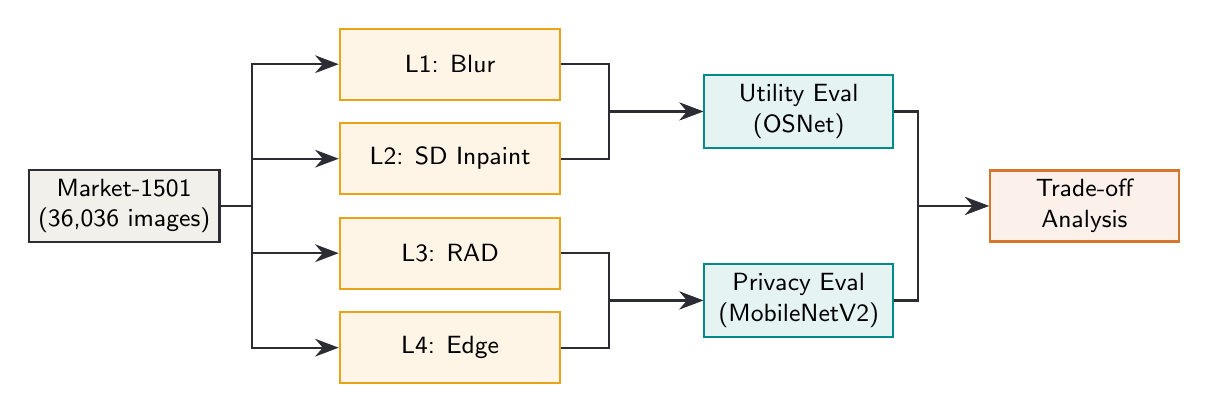
\begin{tikzpicture}[
        node distance=0.6cm and 1.2cm,
        box/.style={rectangle, draw=cfDark, fill=cfLightGray, thick, minimum height=0.9cm, minimum width=2.4cm, align=center, font=\small},
        anonbox/.style={rectangle, draw=cfAmber, fill=cfCream, thick, minimum height=0.9cm, minimum width=2.8cm, align=center, font=\small},
        evalbox/.style={rectangle, draw=cfTeal, fill=cfTeal!10, thick, minimum height=0.9cm, minimum width=2.4cm, align=center, font=\small},
        resultbox/.style={rectangle, draw=cfOrange, fill=cfOrange!10, thick, minimum height=0.9cm, minimum width=2.4cm, align=center, font=\small},
        arr/.style={-{Stealth[length=3mm]}, thick, cfDark},
    ]
        % Input
        \node[box] (input) {Market-1501\\(36,036 images)};

        % Anonymization levels
        \node[anonbox, right=1.5cm of input, yshift=1.8cm]  (l1) {L1: Blur};
        \node[anonbox, right=1.5cm of input, yshift=0.6cm]  (l2) {L2: SD Inpaint};
        \node[anonbox, right=1.5cm of input, yshift=-0.6cm] (l3) {L3: RAD};
        \node[anonbox, right=1.5cm of input, yshift=-1.8cm] (l4) {L4: Edge};

        % Evaluation
        \node[evalbox, right=1.8cm of l2, yshift=0.6cm]  (utility) {Utility Eval\\(OSNet)};
        \node[evalbox, right=1.8cm of l3, yshift=-0.6cm]   (privacy) {Privacy Eval\\(MobileNetV2)};

        % Output
        \node[resultbox, right=1.2cm of utility, yshift=-1.2cm] (result) {Trade-off\\Analysis};

        % Arrows: input -> levels
        \draw[arr] (input.east) -- ++(0.4,0) |- (l1.west);
        \draw[arr] (input.east) -- ++(0.4,0) |- (l2.west);
        \draw[arr] (input.east) -- ++(0.4,0) |- (l3.west);
        \draw[arr] (input.east) -- ++(0.4,0) |- (l4.west);

        % Arrows: levels -> evaluations
        \draw[arr] (l1.east) -- ++(0.6,0) |- (utility.west);
        \draw[arr] (l2.east) -- ++(0.6,0) |- (utility.west);
        \draw[arr] (l3.east) -- ++(0.6,0) |- (privacy.west);
        \draw[arr] (l4.east) -- ++(0.6,0) |- (privacy.west);

        % Arrows: evaluations -> result
        \draw[arr] (utility.east) -- ++(0.3,0) |- (result.west);
        \draw[arr] (privacy.east) -- ++(0.3,0) |- (result.west);

    \end{tikzpicture}
    \caption{ANON4REID evaluation pipeline. Each anonymized dataset variant is evaluated for both utility (OSNet \acrshort{reid} performance) and privacy (MobileNetV2 attacker accuracy).}
    \label{fig:pipeline}
\end{figure}

The anonymization levels are ordered by intended privacy strength:

\begin{table}[H]
    \centering
    \begin{tabular}{@{}clll@{}}
        \toprule
        \rowcolor{cfTeal} \thdr{Level} & \thdr{Name} & \thdr{Technique} & \thdr{Scope} \\
        \midrule
        L1 & Gaussian Blur & MediaPipe face detection + blur & Face region \\
        L2 & SD Inpaint & Stable Diffusion inpainting & Central torso \\
        L3 & RAD & ControlNet OpenPose + SD v1.5 & Full body replacement \\
        L4 & Edge Silhouette & Canny edge detection & Entire image \\
        \bottomrule
    \end{tabular}
    \caption{Summary of the four anonymization levels.}
    \label{tab:anon_levels}
\end{table}


\section{Anonymization Pipeline}

\subsection{Level 1: Gaussian Blur with Face Detection}

Level~1 applies Gaussian blur (kernel size $15 \times 15$, $\sigma = 30$) to the face region of each pedestrian image. Face localization uses the MediaPipe Face Detection model \cite{lugaresi2019mediapipe}, specifically the short-range model variant with a minimum detection confidence threshold of 0.3.

Because Market-1501 images are only 64$\times$128 pixels, face detection frequently fails due to insufficient resolution. A spatial fallback is therefore implemented: when MediaPipe returns no detections, the blur is applied to a heuristically defined head region covering the top 28\% of the image height and the central 70\% of the image width (from 15\% to 85\%). This fallback is based on the observation that Market-1501 bounding boxes are consistently cropped around the full body, placing the head in the upper portion of the frame.

\begin{equation}
    \text{ROI}_\text{fallback} = \text{image}[0 : \lfloor 0.28 \cdot H \rfloor,\; \lfloor 0.15 \cdot W \rfloor : \lfloor 0.85 \cdot W \rfloor]
    \label{eq:blur_fallback}
\end{equation}

An alternative design would apply the upscale--process--downscale pipeline (Section~\ref{sec:resolution}) to Level~1, giving MediaPipe higher-resolution input for face detection. This approach was considered and rejected for several reasons:

\begin{enumerate}[noitemsep]
    \item Lanczos upscaling interpolates between existing pixels without adding genuine facial detail. The upscaled ``face'' remains a smoothed approximation of the 64$\times$128 original, so MediaPipe may still fail on synthetic features that lack real structure.
    \item The spatial fallback already produces reasonable results for Market-1501 specifically, because the dataset's bounding boxes are consistently cropped around full-body pedestrians with heads centered in the upper portion of the frame.
    \item Adding upscaling would introduce per-image resize overhead to what is intended to be the lightweight, CPU-bound anonymization level. Part of Level~1's value in the benchmark is its minimal computational cost.
    \item More accurate face detection could produce tighter blur regions than the current fallback crop. A smaller blurred area might actually \textit{increase} facial information leakage at the region boundaries compared to the more conservative heuristic crop.
    \item The core finding is unaffected: the attacker exploits body-level features (clothing, shape, accessories) that face blurring leaves untouched regardless of localization precision. The 88.66\% identity leakage would persist even with perfect face detection.
\end{enumerate}


\subsection{Resolution Handling}
\label{sec:resolution}

Market-1501 images are natively 64$\times$128 pixels, far below the minimum resolution required by generative models. To address this, Levels~2 and~3 apply an upscale--process--downscale pipeline: each image is resized from 64$\times$128 to 256$\times$512 using Lanczos interpolation, the generative model operates on the upscaled image, and the output is resized back to 64$\times$128. This ensures coherent generative output while maintaining data compatibility with the original dataset structure.


\subsection{Level 2: Stable Diffusion Inpainting}

Level~2 uses the \texttt{sd-legacy/stable-diffusion-inpainting} model \cite{rombach2022ldm} to replace the central torso region with AI-generated content. A geometric binary mask covers the central 60\% width and 80\% height of the image (from 20\% to 80\% width, 10\% to 90\% height), targeting the body region that carries the most discriminative appearance features.

The inpainting model is conditioned on two text prompts:
\begin{itemize}[noitemsep]
    \item \textbf{Prompt:} \texttt{"empty background, no person, floor, wall"}
    \item \textbf{Negative prompt:} \texttt{"person, human, body, blurry, distorted"}
\end{itemize}

Inference uses 20 denoising steps with a guidance scale of 7.5. Each image is upscaled before processing and downscaled back afterward (Section~\ref{sec:resolution}).

\subsection{Level 3: Realistic Anonymization by Diffusion (RAD)}

Level~3 replaces the original person entirely with a synthetically generated individual who preserves the original body pose but shares no visual identity features. The pipeline consists of three components:

\begin{enumerate}[noitemsep]
    \item \textbf{Pose Extraction:} OpenPose \cite{cao2017openpose} extracts a skeleton representation of the person's body joints from the upscaled image, providing a privacy-preserving conditioning signal.
    \item \textbf{Conditioned Generation:} Stable Diffusion v1.5 \cite{rombach2022ldm} with ControlNet OpenPose conditioning \cite{zhang2023controlnet} generates a new person image guided by the extracted skeleton.
    \item \textbf{Inference Acceleration:} LCM-LoRA \cite{luo2023lcm} reduces the required denoising steps from 50 to 8, making batch processing of 36,036 images practical.
\end{enumerate}

The generation uses a guidance scale of 1.5 and a ControlNet conditioning scale of 0.8, with the prompt \texttt{"a person, different appearance, full body, high quality, realistic"}.

\subsection{Level 4: Canny Edge Detection}

Level~4 applies Canny edge detection \cite{canny1986edge} with thresholds $(T_\text{low}, T_\text{high}) = (100, 200)$ to the entire image, converting it to a binary edge map. The single-channel output is replicated to three channels (RGB) for compatibility with downstream models. This technique strips all color, texture, and fine-grained appearance information, retaining only structural contours.


\section{Evaluation Framework}

\textbf{Utility} is measured by the \acrshort{reid} performance of a pre-trained \acrshort{osnet} (\texttt{osnet\_x1\_0}) model evaluated on each anonymized dataset variant. The evaluation follows the standard closed-set \acrshort{reid} protocol: features are extracted from all query and gallery images as 512-dimensional embeddings, a Euclidean distance matrix is computed between all query--gallery pairs, and k-reciprocal encoding re-ranking \cite{zhong2017reranking} is applied to refine the distance matrix before computing \acrshort{cmc} curves and \acrshort{map} using the \texttt{torchreid} evaluation function with a maximum rank of 50. Each anonymized dataset variant is dynamically registered as a \texttt{torchreid} dataset using Python's \texttt{type()} to create subclasses of \texttt{Market1501} with modified directory paths, ensuring full compatibility with the standard evaluation pipeline without requiring custom dataloaders.

\textbf{Privacy} is measured by the Top-1 accuracy of an adversarial MobileNetV2 \cite{sandler2018mobilenetv2} classifier on anonymized query images. The attacker is pre-trained on ImageNet \cite{deng2009imagenet} and fine-tuned on original (non-anonymized) Market-1501 images to classify person identity. During inference, each anonymized query image is resized to 256$\times$128 pixels and normalized using the ImageNet channel statistics ($\mu = [0.485, 0.456, 0.406]$, $\sigma = [0.229, 0.224, 0.225]$) before being passed through the classifier. The privacy metric is:

\begin{equation}
    \text{Privacy Leakage} = \frac{\text{Correctly classified query images}}{\text{Total query images}} \times 100\%
    \label{eq:privacy_leak}
\end{equation}

A high leakage value indicates that the anonymization technique fails to protect identity information; a value near 0\% indicates strong privacy protection. For context, random guessing across 750 identity classes would yield approximately $\frac{1}{750} \times 100\% \approx 0.13\%$ accuracy, providing a theoretical floor for the privacy metric.

The attacker is trained on the \texttt{bounding\_box\_test} split (750 identities, 19,732 images) rather than \texttt{bounding\_box\_train}. This is because Market-1501's training and test/query sets have \textbf{completely disjoint identity sets} (751 vs.\ 750 IDs). Training on the training split would yield 0\% accuracy on query images regardless of anonymization, since none of the training identities appear in the query set. By training on the test split, which shares the same 750 identities as the query set, the attacker can meaningfully classify query images, and its accuracy drop on anonymized queries isolates the effect of the anonymization technique from the identity partition boundary.

\textbf{Trade-off.} The central analysis jointly examines utility degradation and privacy gain across anonymization levels. An effective anonymization technique should minimize utility loss while maximizing privacy protection. We define the \textit{Effectiveness Index} as:

\begin{equation}
    \text{Effectiveness Index} = \frac{\text{Privacy Protection (\%)}}{100 - \text{Utility (mAP \%)}}
    \label{eq:effectiveness}
\end{equation}

This ratio captures how much privacy is gained per unit of utility sacrificed. A higher value indicates a more efficient trade-off, while a low value indicates that privacy was gained at disproportionate utility cost.

    \chapter{Implementation}

\section{Project Scope and Evolution}

The project was initially scoped as a dual-track investigation: a \textbf{self-trained track}, in which an OSNet model would be trained from scratch on the Market-1501 training set and then evaluated on anonymized variants, and a \textbf{pretrained track}, using established pretrained weights from \texttt{torchreid}. The self-trained track was intended to investigate whether a model trained on original data would exhibit different sensitivity to anonymization compared to a model trained with standardized augmentation and hyperparameter tuning.

During development, the self-trained track deviated significantly from the core research question. Training a \acrshort{reid} model from scratch introduced a substantial set of secondary concerns: hyperparameter tuning (learning rate schedules, batch sizes, sampling strategies), architecture selection, training data augmentation, convergence validation, and the need to establish that the self-trained model was a fair comparator before any anonymization analysis could begin. These issues consumed development time without contributing directly to the privacy--utility trade-off investigation, which is the primary focus of this project.

The decision was made to \textbf{rescope to the pretrained track only}. This refocusing provided several advantages: (a)~the pretrained \texttt{osnet\_x1\_0} weights from \texttt{torchreid} represent a well-validated, reproducible baseline that isolates the anonymization effect from model training noise, (b)~development effort could be redirected toward building a comprehensive four-level anonymization pipeline and a thorough evaluation framework, and (c)~the results are directly comparable to published \acrshort{reid} benchmarks that use the same pretrained model.

Table~\ref{tab:timeline} summarizes the project phases.

\begin{table}[H]
    \centering
    \begin{tabular}{@{}clp{8cm}@{}}
        \toprule
        \rowcolor{cfTeal} \thdr{Phase} & \thdr{Title} & \thdr{Description} \\
        \midrule
        1 & Initial Scoping & Defined research questions. Planned dual-track approach (self-trained + pretrained OSNet). Identified Market-1501 as the benchmark dataset. \\
        2 & Anonymization Pipeline & Implemented L1 (blur) and L4 (edge) as CPU-bound methods. Developed the resolution-handling pipeline. Implemented L2 (SD Inpainting) and L3 (RAD) on Kaggle GPU notebooks. \\
        3 & Scope Revision & Self-trained track encountered significant scope deviation. Rescoped to pretrained OSNet only to focus on the core privacy--utility trade-off analysis. \\
        4 & Evaluation Framework & Deployed pretrained OSNet for utility evaluation. Trained MobileNetV2 attacker for privacy evaluation. Regenerated L1 dataset with upgraded MediaPipe face detection. \\
        5 & Integration & Built Streamlit dashboard. Compiled trade-off analysis, visualizations, and final report. \\
        \bottomrule
    \end{tabular}
    \caption{Project development phases.}
    \label{tab:timeline}
\end{table}


\section{Development Environment}

All experiments were conducted on a system with an AMD Ryzen 5 7600X CPU (6 cores), AMD Radeon RX 7800 XT GPU (16~GB VRAM), Python 3.12, and PyTorch 2.11.0 with ROCm/HIP backend (\texttt{device="cuda"} mapped transparently to HIP via the ROCm compatibility layer). GPU-bound dataset generation (Levels~2 and~3) was initially performed on Kaggle's free GPU tier (NVIDIA Tesla P100, 16~GB VRAM) before local hardware was available. Table~\ref{tab:dependencies} lists the principal libraries.

\begin{table}[H]
    \centering
    \begin{tabular}{@{}lll@{}}
        \toprule
        \rowcolor{cfTeal} \thdr{Library} & \thdr{Version} & \thdr{Purpose} \\
        \midrule
        torchreid & 0.2.5 & ReID model management and evaluation \\
        diffusers & 0.37.1 & Stable Diffusion pipelines \\
        controlnet-aux & 0.0.10 & OpenPose skeleton extraction \\
        mediapipe & 0.10.35 & Face detection (Level~1) \\
        torchvision & 0.26.0 & MobileNetV2 and image transforms \\
        opencv-python & 4.13.0 & Image processing and Canny edge detection \\
        streamlit & 1.45.0 & Interactive dashboard \\
        plotly & 6.1.2 & Interactive chart visualizations \\
        \bottomrule
    \end{tabular}
    \caption{Principal software dependencies.}
    \label{tab:dependencies}
\end{table}


\section{Dataset Generation}

The four anonymized dataset variants were generated by applying each anonymization function to all images in the three Market-1501 splits (\texttt{bounding\_box\_train}, \texttt{bounding\_box\_test}, and \texttt{query}), producing approximately 36,000 anonymized images per level. Each anonymized dataset preserves the original Market-1501 directory structure and filename conventions, ensuring compatibility with the \texttt{torchreid} data loading pipeline.

Gaussian blur (Level~1) and Canny edge detection (Level~4) are CPU-bound operations and were initially generated on Kaggle's free tier in approximately 15 minutes each. The Level~1 dataset was subsequently regenerated locally using the upgraded MediaPipe face detection implementation, which replaced an earlier OpenCV Haar cascade approach that exhibited lower detection accuracy on the small 64$\times$128 images.

Stable Diffusion inpainting (Level~2) and RAD (Level~3) require \acrshort{gpu} acceleration and were generated using Kaggle \acrshort{gpu} notebooks. These levels apply the upscale--process--downscale pipeline described in Section~\ref{sec:resolution}, processing each image individually through the generative model. Due to the sequential nature of diffusion inference, generation of each GPU-bound dataset required several hours of processing time across the full 36,036 images.


\section{Attacker Model Training}

The MobileNetV2 identity classifier was fine-tuned on the original (non-anonymized) \texttt{bounding\_box\_test} images to learn the visual appearance of each of the 750 test/query identities. Table~\ref{tab:attacker_config} details the training configuration.

\begin{table}[H]
    \centering
    \begin{tabular}{@{}ll@{}}
        \toprule
        \rowcolor{cfTeal} \thdr{Parameter} & \thdr{Value} \\
        \midrule
        Base model & MobileNetV2 (ImageNet pre-trained) \\
        Training data & \texttt{bounding\_box\_test} (19,732 images, 750 IDs) \\
        Input resolution & 256$\times$128 pixels \\
        Final layer & Linear(1280, 750) \\
        Loss function & CrossEntropyLoss \\
        Optimizer & Adam ($\text{lr} = 3 \times 10^{-4}$) \\
        Batch size & 64 \\
        Max epochs & 30 \\
        Early stopping & Patience = 4 (on training loss) \\
        \bottomrule
    \end{tabular}
    \caption{MobileNetV2 attacker training configuration.}
    \label{tab:attacker_config}
\end{table}

Identity labels are parsed from Market-1501 filenames (the first four characters encode the person ID). Images with IDs $-1$ (junk) and $0000$ (distractor) are excluded from training. The final layer of MobileNetV2 is replaced with a linear classifier mapping the 1280-dimensional feature vector to 750 identity classes. All layers are fine-tuned (not frozen), allowing the ImageNet-pretrained features to adapt to the pedestrian identity classification task.


\section{Interactive Dashboard}

A Streamlit-based dashboard (\texttt{app.py}) provides interactive exploration of the experimental results across three tabs. The \textbf{Trade-off Analysis} tab presents dual-axis charts comparing mAP and privacy leakage, scatter plots mapping the privacy--utility space, and per-level metric summary cards. The \textbf{Visual Comparison} tab displays side-by-side query images across all anonymization levels, allowing visual inspection of how each technique transforms the original image. The \textbf{Detailed Metrics} tab provides \acrshort{cmc} curve charts, mAP waterfall diagrams, a heatmap of all metrics across levels, and a full data table for export. All charts use Plotly with the \texttt{plotly\_white} template and the Cassette Futurism color palette for visual consistency with this report.

    \chapter{Results}

\section{Utility Evaluation}

The pre-trained \acrshort{osnet} (\texttt{osnet\_x1\_0}) model was evaluated on the original Market-1501 dataset and all anonymized variants using k-reciprocal encoding re-ranking \cite{zhong2017reranking} applied to the Euclidean distance matrix. Table~\ref{tab:baseline} reports the baseline performance, confirming that the pretrained model achieves Rank-1 accuracy of 92.04\% and mAP of 86.23\% with re-ranking, consistent with published results for \texttt{osnet\_x1\_0}. These values serve as the reference against which all anonymized variants are compared. Table~\ref{tab:utility} reports the anonymized results.

\begin{table}[H]
    \centering
    \begin{tabular}{@{}lc@{}}
        \toprule
        \rowcolor{cfTeal} \thdr{Metric} & \thdr{Value} \\
        \midrule
        mAP & 0.8623 \\
        Rank-1 & 0.9204 \\
        Rank-5 & 0.9469 \\
        Rank-10 & 0.9587 \\
        Rank-20 & 0.9694 \\
        \bottomrule
    \end{tabular}
    \caption{Baseline \acrshort{osnet} performance on the original Market-1501 dataset.}
    \label{tab:baseline}
\end{table}

\begin{table}[H]
    \centering
    \begin{tabular}{@{}lccccc@{}}
        \toprule
        \rowcolor{cfTeal} \thdr{Level} & \thdr{mAP} & \thdr{Rank-1} & \thdr{Rank-5} & \thdr{Rank-10} & \thdr{Rank-20} \\
        \midrule
        L1: Blur & 0.6976 & 0.8070 & 0.8809 & 0.9008 & 0.9264 \\
        L2: SDInpaint & 0.0198 & 0.0546 & 0.1339 & 0.1719 & 0.2227 \\
        L3: RAD & 0.0015 & 0.0006 & 0.0050 & 0.0101 & 0.0202 \\
        L4: Edge & 0.0114 & 0.0235 & 0.0600 & 0.0855 & 0.1191 \\
        \bottomrule
    \end{tabular}
    \caption{Utility results: \acrshort{osnet} \acrshort{reid} performance across anonymization levels.}
    \label{tab:utility}
\end{table}

L1 (Blur) retains 80.9\% of baseline mAP (0.6976 vs.\ 0.8623), indicating that face-only blurring preserves the body-level features that \acrshort{osnet} primarily relies on for cross-camera matching. The Rank-1 accuracy of 80.70\% means that four out of five queries still retrieve the correct identity as the top result despite face anonymization. L2 (SDInpaint) drops mAP to 2.3\% of baseline (0.0198), confirming that replacing the central torso region destroys most discriminative features. L3 (RAD) produces the most severe degradation at 0.17\% of baseline (mAP = 0.0015), as full-body replacement generates entirely new appearances with no identity correlation to the original. L4 (Edge) retains slightly more utility than RAD at 1.3\% of baseline (mAP = 0.0114), because preserved edge structure encodes some body-shape information that enables marginally better matching. Figure~\ref{fig:map_comparison} visualizes the mAP degradation; Figure~\ref{fig:cmc_curves} compares the \acrlong{cmc} curves across all levels, showing that L1 closely tracks the baseline while L2--L4 remain near zero across all rank thresholds.

\begin{figure}[H]
    \centering
    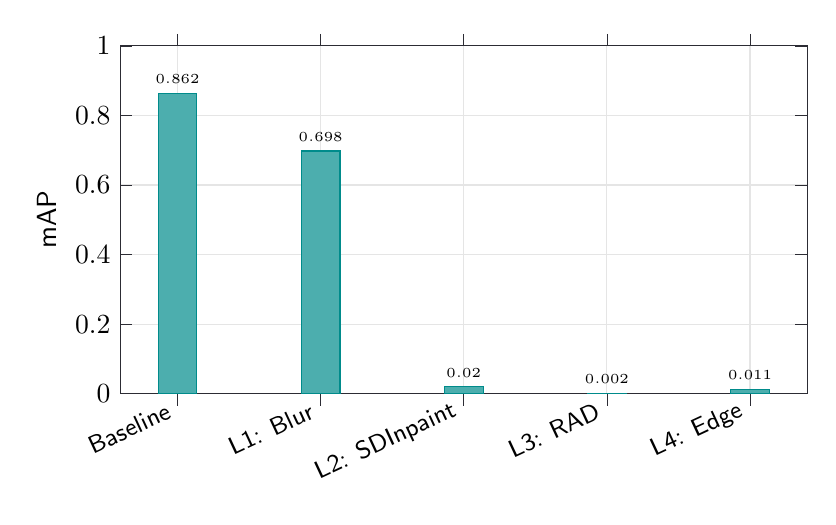
\begin{tikzpicture}
        \begin{axis}[
            ybar,
            width=0.85\columnwidth,
            height=6cm,
            bar width=14pt,
            ylabel={mAP},
            symbolic x coords={Baseline, L1: Blur, L2: SDInpaint, L3: RAD, L4: Edge},
            xtick=data,
            xticklabel style={rotate=25, anchor=east, font=\small},
            ymin=0, ymax=1.0,
            nodes near coords,
            nodes near coords style={font=\tiny, above},
            every node near coord/.append style={/pgf/number format/.cd, fixed, precision=3},
            grid=major,
            grid style={gray!20},
            axis line style={cfDark},
            tick style={cfDark},
        ]
            \addplot[fill=cfTeal!70, draw=cfTeal] coordinates {
                (Baseline, 0.8623)
                (L1: Blur, 0.6976)
                (L2: SDInpaint, 0.0198)
                (L3: RAD, 0.0015)
                (L4: Edge, 0.0114)
            };
        \end{axis}
    \end{tikzpicture}
    \caption{Mean Average Precision (mAP) across anonymization levels. Baseline represents the original Market-1501 dataset evaluated with OSNet.}
    \label{fig:map_comparison}
\end{figure}

\begin{figure}[H]
    \centering
    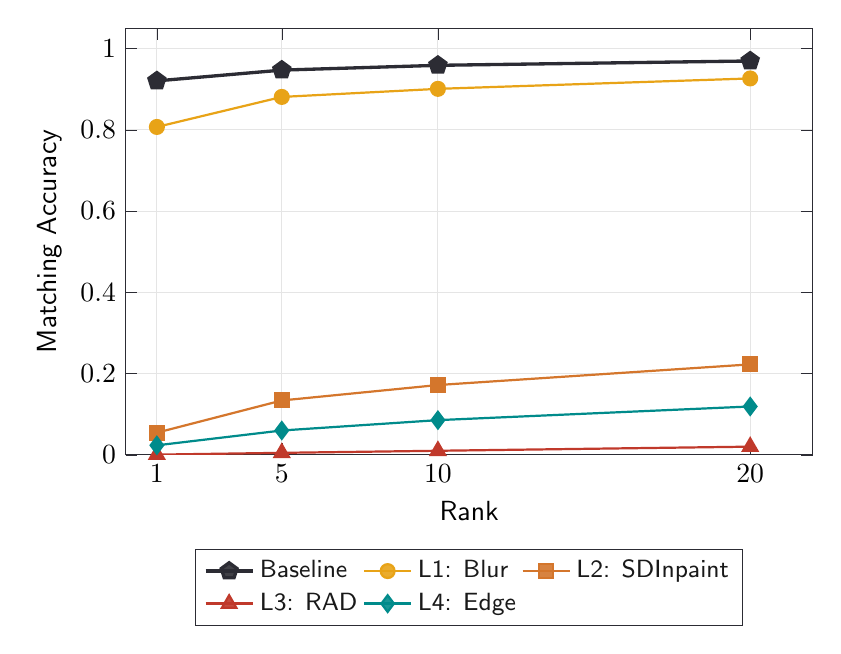
\begin{tikzpicture}
        \begin{axis}[
            width=0.85\columnwidth,
            height=7cm,
            xlabel={Rank},
            ylabel={Matching Accuracy},
            xmin=0, xmax=22,
            ymin=0, ymax=1.05,
            xtick={1,5,10,20},
            grid=major,
            grid style={gray!20},
            axis line style={cfDark},
            tick style={cfDark},
            legend style={at={(0.5,-0.22)}, anchor=north, font=\small, fill=white, fill opacity=0.9, draw=cfDark, legend columns=3},
            legend cell align=left,
        ]
            \addplot[cfDark, very thick, mark=pentagon*, mark size=3pt]
                coordinates {(1,0.9204) (5,0.9469) (10,0.9587) (20,0.9694)};
            \addlegendentry{Baseline}

            \addplot[cfAmber, thick, mark=*, mark size=2.5pt]
                coordinates {(1,0.8070) (5,0.8809) (10,0.9008) (20,0.9264)};
            \addlegendentry{L1: Blur}

            \addplot[cfOrange, thick, mark=square*, mark size=2.5pt]
                coordinates {(1,0.0546) (5,0.1339) (10,0.1719) (20,0.2227)};
            \addlegendentry{L2: SDInpaint}

            \addplot[cfRed, thick, mark=triangle*, mark size=3pt]
                coordinates {(1,0.0006) (5,0.0050) (10,0.0101) (20,0.0202)};
            \addlegendentry{L3: RAD}

            \addplot[cfTeal, thick, mark=diamond*, mark size=3pt]
                coordinates {(1,0.0235) (5,0.0600) (10,0.0855) (20,0.1191)};
            \addlegendentry{L4: Edge}
        \end{axis}
    \end{tikzpicture}
    \caption{\acrlong{cmc} curves for all anonymization levels and the baseline. L1 (Blur) closely tracks the Baseline, while L2--L4 remain near zero across all ranks.}
    \label{fig:cmc_curves}
\end{figure}


\section{Privacy Evaluation}

Table~\ref{tab:privacy} presents the identity classification accuracy of the MobileNetV2 attacker on each anonymized query set (3,368 query images, excluding junk and distractor images).

\begin{table}[H]
    \centering
    \begin{tabular}{@{}lccc@{}}
        \toprule
        \rowcolor{cfTeal} \thdr{Level} & \thdr{Top-1 Accuracy (\%)} & \thdr{Correct} & \thdr{Total} \\
        \midrule
        L1: Blur & 88.66 & 2,986 & 3,368 \\
        L2: SDInpaint & 11.76 & 396 & 3,368 \\
        L4: Edge & 0.15 & 5 & 3,368 \\
        L3: RAD & 0.15 & 5 & 3,368 \\
        \bottomrule
    \end{tabular}
    \caption{Privacy results: MobileNetV2 attacker Top-1 accuracy on anonymized query images. Lower accuracy indicates stronger privacy protection.}
    \label{tab:privacy}
\end{table}

L1 provides minimal privacy protection: 88.66\% leakage means the attacker correctly identifies 2,986 of 3,368 query individuals despite face blurring, confirming that MobileNetV2 learns to rely on body-level features (clothing, body shape, accessories) rather than facial features alone. For reference, random guessing across 750 identity classes would yield approximately 0.13\% accuracy. L2 reduces leakage to 11.76\% (396 correct), a substantial improvement attributable to the destruction of torso-level features; the residual leakage likely corresponds to images where the inpainting mask did not fully cover discriminative features at image boundaries. L3 (RAD) and L4 (Edge) both achieve 0.15\% leakage (5 out of 3,368), which is statistically indistinguishable from random chance given 750 classes, effectively confirming that these techniques reduce the attacker to guessing. Figure~\ref{fig:privacy_leakage} visualizes the identity leakage.

\begin{figure}[H]
    \centering
    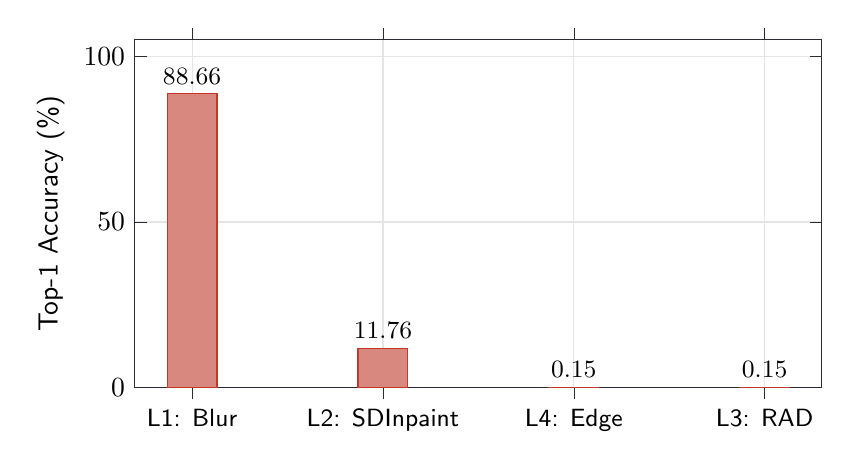
\begin{tikzpicture}
        \begin{axis}[
            ybar,
            width=0.85\columnwidth,
            height=6cm,
            bar width=18pt,
            ylabel={Top-1 Accuracy (\%)},
            symbolic x coords={L1: Blur, L2: SDInpaint, L4: Edge, L3: RAD},
            xtick=data,
            xticklabel style={font=\small},
            ymin=0, ymax=105,
            nodes near coords,
            nodes near coords style={font=\small, above},
            every node near coord/.append style={/pgf/number format/.cd, fixed, precision=2, fixed zerofill},
            grid=major,
            grid style={gray!20},
            axis line style={cfDark},
            tick style={cfDark},
        ]
            \addplot[fill=cfRed!60, draw=cfRed] coordinates {
                (L1: Blur, 88.66)
                (L2: SDInpaint, 11.76)
                (L4: Edge, 0.15)
                (L3: RAD, 0.15)
            };
        \end{axis}
    \end{tikzpicture}
    \caption{Privacy leakage (MobileNetV2 attacker Top-1 accuracy) across anonymization levels. L3 (RAD) and L4 (Edge) reduce the attacker to near-random performance.}
    \label{fig:privacy_leakage}
\end{figure}


\section{Privacy--Utility Trade-off}

Table~\ref{tab:tradeoff} summarizes the combined privacy--utility metrics.

\begin{table}[H]
    \centering
    \begin{tabular}{@{}lcccc@{}}
        \toprule
        \rowcolor{cfTeal} \thdr{Level} & \thdr{mAP} & \thdr{Leak (\%)} & \thdr{Protection (\%)} & \thdr{mAP \% of BL} \\
        \midrule
        Baseline & 0.8623 & n/a & n/a & 100.0 \\
        L1: Blur & 0.6976 & 88.66 & 11.34 & 80.9 \\
        L2: SDInpaint & 0.0198 & 11.76 & 88.24 & 2.3 \\
        L3: RAD & 0.0015 & 0.15 & 99.85 & 0.17 \\
        L4: Edge & 0.0114 & 0.15 & 99.85 & 1.3 \\
        \bottomrule
    \end{tabular}
    \caption{Combined privacy--utility trade-off summary. ``Leak'' is the attacker's Top-1 accuracy; ``Protection'' is $100 - \text{Leak}$; ``mAP \% of BL'' is the fraction of baseline mAP retained.}
    \label{tab:tradeoff}
\end{table}

The trade-off reveals a sharp cliff rather than a gradual continuum. L1 retains most utility (mAP = 0.6976, 80.9\% of baseline) but provides almost no privacy (88.66\% leakage, only 11.34\% protection). L2 crosses the cliff: it achieves substantial privacy (88.24\% protection) but at steep utility cost (mAP drops to 0.0198, retaining only 2.3\% of baseline). L3 and L4 achieve near-perfect privacy (99.85\% protection) with near-zero utility (mAP $< 0.02$). No ``sweet spot'' was found where reasonable privacy coexists with acceptable utility: there is no evaluated configuration where, for example, 50\% privacy protection accompanies 50\% utility retention. This suggests that the features required for \acrshort{reid} (clothing appearance, body proportions, carried objects) and those revealing identity to a classifier overlap substantially, making the trade-off inherently discontinuous rather than smoothly adjustable. Figure~\ref{fig:tradeoff_scatter} plots this relationship, with the empty ``Ideal Zone'' (bottom-right: high utility, low leakage) visually confirming the absence of a favorable operating point.

\begin{figure}[H]
    \centering
    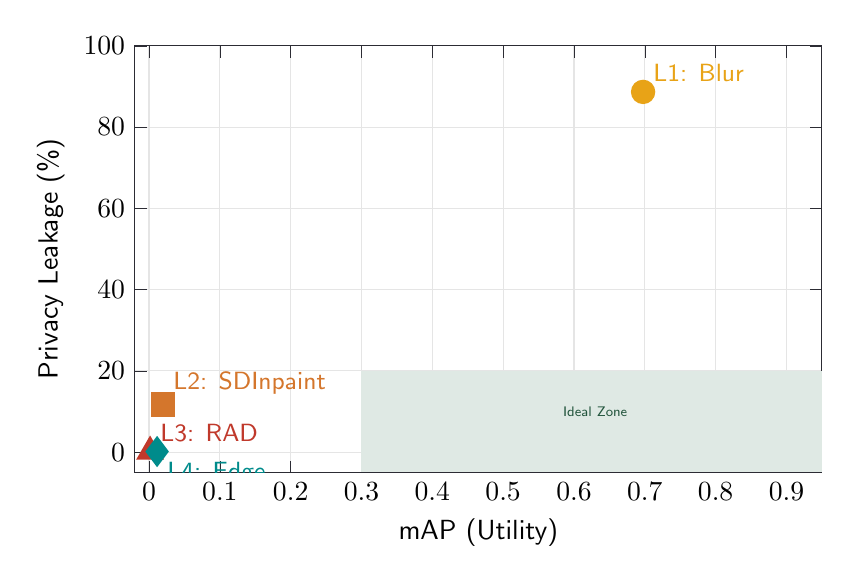
\begin{tikzpicture}
        \begin{axis}[
            width=0.85\columnwidth,
            height=7cm,
            xlabel={mAP (Utility)},
            ylabel={Privacy Leakage (\%)},
            xmin=-0.02, xmax=0.95,
            ymin=-5, ymax=100,
            grid=major,
            grid style={gray!20},
            axis line style={cfDark},
            tick style={cfDark},
            legend pos=north east,
            legend style={font=\small},
        ]
            % Ideal zone shading (high utility, low leakage)
            \fill[cfGreen!15] (axis cs:0.3,-5) rectangle (axis cs:0.95,20);
            \node[font=\tiny, cfGreen!80!black] at (axis cs:0.63,10) {Ideal Zone};

            \addplot[only marks, mark=*, mark size=4pt, cfAmber, thick]
                coordinates {(0.6976, 88.66)} node[above right, font=\small] {L1: Blur};
            \addplot[only marks, mark=square*, mark size=4pt, cfOrange, thick]
                coordinates {(0.0198, 11.76)} node[above right, font=\small] {L2: SDInpaint};
            \addplot[only marks, mark=triangle*, mark size=5pt, cfRed, thick]
                coordinates {(0.0015, 0.15)} node[above right, font=\small] {L3: RAD};
            \addplot[only marks, mark=diamond*, mark size=5pt, cfTeal, thick]
                coordinates {(0.0114, 0.15)} node[below right, font=\small] {L4: Edge};
        \end{axis}
    \end{tikzpicture}
    \caption{Privacy--utility trade-off scatter plot. The ideal zone (high utility, low leakage) in the bottom-right is unoccupied, illustrating the fundamental tension between privacy and \acrshort{reid} utility.}
    \label{fig:tradeoff_scatter}
\end{figure}


\section{Effect of K-Reciprocal Re-Ranking}

All utility results reported above use k-reciprocal encoding \cite{zhong2017reranking} as a post-processing step on the Euclidean distance matrix. This technique refines the initial ranking by exploiting the k-reciprocal nearest neighbor structure: if two images are mutual nearest neighbors, their distance is reinforced; if not, it is penalized. Re-ranking operates entirely at evaluation time and requires no model retraining.

An initial evaluation was conducted without re-ranking, using raw Euclidean distance retrieval only. Table~\ref{tab:reranking_comparison} compares the mAP results before and after applying k-reciprocal encoding.

\begin{table}[H]
    \centering
    \begin{tabular}{@{}lccc@{}}
        \toprule
        \rowcolor{cfTeal} \thdr{Level} & \thdr{mAP (w/o)} & \thdr{mAP (w/)} & \thdr{$\Delta$ mAP} \\
        \midrule
        Baseline & 0.5720 & 0.8623 & +0.2903 \\
        L1: Blur & 0.3942 & 0.6976 & +0.3034 \\
        L2: SDInpaint & 0.0172 & 0.0198 & +0.0026 \\
        L3: RAD & 0.0015 & 0.0015 & +0.0000 \\
        L4: Edge & 0.0093 & 0.0114 & +0.0021 \\
        \bottomrule
    \end{tabular}
    \caption{Effect of k-reciprocal re-ranking on mAP. ``w/o'' = without re-ranking (raw Euclidean); ``w/'' = with k-reciprocal encoding.}
    \label{tab:reranking_comparison}
\end{table}

Re-ranking produces substantial improvements for the Baseline (+0.2903 mAP) and L1 (+0.3034 mAP), where the feature embeddings contain sufficient discriminative information for the k-reciprocal neighbor structure to be meaningful. For L2--L4, the improvement is negligible ($\Delta < 0.003$) because the anonymization has destroyed the identity-bearing features to such a degree that no post-processing on the distance matrix can recover useful ranking information. This confirms that the privacy--utility cliff is robust to the choice of retrieval strategy: re-ranking amplifies the absolute gap between L1 and L2--L4 but does not alter the fundamental cliff structure.

    \chapter{Discussion}

\section{Key Findings}

The experimental results reveal several significant patterns in the relationship between anonymization, privacy, and re-identification utility.

\textbf{Face Blurring is Insufficient for Privacy.}
Level~1 (Gaussian blur on the face region) provides virtually no privacy protection against a learned attacker. The MobileNetV2 classifier achieves 88.66\% Top-1 accuracy on face-blurred images, compared to a random-guessing baseline of $\frac{1}{750} \approx 0.13\%$ for 750 identity classes. This result demonstrates that identity classification models can exploit clothing texture, body shape, carried objects, and other non-facial appearance cues that face blurring leaves intact. The high leakage persists because \acrshort{cnn} classifiers are not limited to human-interpretable features: they learn discriminative patterns across the entire spatial extent of the input image, including correlations between background context, clothing color distributions, and body proportions.

\begin{keybox}[Practical Implication]
Face blurring, the most commonly deployed anonymization technique in real-world surveillance systems, may create a false sense of privacy compliance when adversaries have access to modern deep learning classifiers. Organizations relying solely on face blurring for GDPR compliance should consider that body-level features remain fully exposed and exploitable.
\end{keybox}

\textbf{The Privacy--Utility Cliff.}
Rather than a smooth, continuous trade-off curve, the results reveal a sharp ``cliff'' between L1 and L2. Level~1 retains 80.9\% of baseline mAP but fails on privacy (88.66\% leakage); Levels~2--4 achieve strong privacy ($\geq$88.24\% protection) but retain less than 2.3\% of baseline mAP. There is no intermediate region where, for example, 50\% privacy protection coexists with 50\% utility retention. This cliff arises because the visual features that make a person re-identifiable across cameras (clothing appearance, body proportions, carried objects) are precisely the same features that an identity classifier exploits. Partial anonymization either leaves these features intact (L1) or destroys them (L2--L4), with no gradual middle ground observable in the evaluated techniques.

\textbf{Generative vs.\ Deterministic Methods.}
SD Inpaint (L2), RAD (L3), and Edge detection (L4) achieve comparable privacy protection ($\geq$88\%) through fundamentally different mechanisms: selective content replacement, full-body synthesis, and structural reduction respectively. L3 and L4 both achieve identical leakage rates of 0.15\% (5 correct classifications out of 3,368 queries), which is consistent with random chance given 750 identity classes. The comparable privacy outcomes across these diverse techniques suggest that the computational cost of generative models may not be justified for privacy protection alone: Canny edge detection achieves the same 0.15\% leakage as the ControlNet-based RAD pipeline at a fraction of the computational cost and without requiring GPU acceleration. The advantage of generative methods lies in utility preservation: L2 retains more structural information (Rank-20 of 22.27\%) than L4 (11.91\%), which may matter in applications where partial re-identification capability is acceptable.

\textbf{Utility Evaluation as an Implicit Privacy Attack.}
The \acrshort{osnet} model used for utility measurement is trained on the Market-1501 training split (751 IDs) with disjoint identities from the test/query split (750 IDs). Because \acrshort{reid} models learn generalizable feature embeddings rather than identity-specific classifiers, \acrshort{osnet} can match unseen identities through nearest-neighbor retrieval in the embedding space. This means the utility metrics (mAP, \acrshort{cmc}) already constitute an implicit embedding-based privacy attack: any query image that is successfully matched to its correct gallery counterpart has been effectively re-identified. The dedicated MobileNetV2 attacker measures a complementary threat model (direct closed-set classification rather than open-set retrieval), so together the two evaluations cover both major attack vectors against anonymized surveillance data.


\section{State-of-the-Art Context}

\textbf{Model positioning.} \acrshort{osnet} (\texttt{osnet\_x1\_0}) \cite{zhou2019osnet} occupies a mid-range position in the current person \acrshort{reid} landscape. The model was chosen for its balance between discriminative power and lightweight architecture (2.2M parameters), making it representative of practical deployment scenarios where computational resources are constrained. Our measured baseline (mAP = 86.23\%, Rank-1 = 92.04\%) uses Euclidean distance retrieval with k-reciprocal encoding re-ranking \cite{zhong2017reranking}, a standard post-processing technique that refines rankings by exploiting mutual nearest-neighbor relationships.

More recent architectures, including vision transformer-based models (e.g., TransReID) and foundation model adaptations (e.g., CLIP-ReID), achieve substantially higher baseline performance on Market-1501 through richer feature representations. Using such models would likely amplify the privacy--utility cliff observed in our experiments: stronger feature extractors capture more identity-discriminative information, meaning (a)~the utility baseline would be higher, (b)~the utility degradation under anonymization would be proportionally larger, and (c)~a stronger implicit privacy attack via the utility metrics would make the privacy challenge more acute. The cliff we observe with a mid-range model therefore represents a \textit{lower bound} on the severity of the trade-off.

\textbf{Privacy evaluation context.} Most prior anonymization studies evaluate privacy through re-identification accuracy alone, treating the utility metric drop as an implicit privacy measure. Our framework separates these concerns by introducing an explicit adversarial identity classifier (MobileNetV2) alongside the \acrshort{reid}-based utility evaluation. This dual-metric approach reveals that face blurring's apparent utility preservation (80.9\% mAP retention) coexists with near-total privacy failure (88.66\% attacker accuracy), a disconnect that a utility-only evaluation would not expose.

\textbf{Anonymization landscape.} The sharp privacy--utility cliff we observe is consistent with findings from related work on privacy in visual data: identity features and task-relevant features are often inseparable when the task itself depends on individual appearance. Our contribution is quantifying this relationship across a spectrum of anonymization techniques on a standardized benchmark, providing empirical evidence that the theoretical tension between privacy and utility manifests as a practical cliff rather than a smooth, negotiable curve.


\section{Limitations and Future Work}

Several limitations should be acknowledged when interpreting these results.

\textbf{Single dataset.} All experiments used Market-1501, which contains low-resolution (64$\times$128) images from six cameras at a single location. The privacy--utility trade-off may differ on higher-resolution datasets (e.g., DukeMTMC-reID, MSMT17) where face detection performs more reliably and generative models produce higher-quality outputs.

\textbf{Single \acrshort{reid} model.} Only \acrshort{osnet} (\texttt{osnet\_x1\_0}) was used for utility evaluation. More recent or larger architectures (e.g., TransReID, CLIP-ReID) with different feature extraction strategies might show different sensitivity to anonymization.

\textbf{Single attacker.} MobileNetV2 represents one specific threat model (supervised classification). Stronger attackers, such as ensemble classifiers, metric learning models, or contrastive learning-based feature extractors, could potentially extract identity information that MobileNetV2 misses, meaning the reported privacy leakage figures represent a lower bound on true vulnerability.

\textbf{Fixed anonymization parameters.} Each level used a single parameter configuration (e.g., kernel size 15, $\sigma = 30$ for L1). Exploring a range of parameter strengths within each level would map the intra-level trade-off curve and potentially identify intermediate configurations.

Future directions include: exploring parametric anonymization strengths within each level to map the cliff transition more precisely; testing against stronger and more diverse attacker models (ensemble classifiers, contrastive learning, few-shot methods); applying the evaluation framework to higher-resolution datasets; and investigating whether privacy-preserving \acrshort{reid} methods can be trained on anonymized data to recover some utility while maintaining privacy guarantees.

    \chapter{Conclusion}

This project presented ANON4REID, a systematic benchmark for evaluating the privacy--utility trade-off in person re-identification on the Market-1501 dataset. Four anonymization techniques of increasing strength were applied across all 36,036 images: Gaussian blur with MediaPipe face detection (L1), Stable Diffusion inpainting (L2), Realistic Anonymization by Diffusion with ControlNet and LCM-LoRA (L3), and Canny edge detection (L4).

Utility was measured by the \acrshort{reid} performance of a pre-trained \acrshort{osnet} model, and privacy was measured by the identity classification accuracy of a MobileNetV2-based adversarial attacker trained on the original test images. The results reveal a stark trade-off:

\begin{keybox}[Summary of Results]
\begin{itemize}[noitemsep]
    \item Face-only blurring (L1) retains 80.9\% of baseline mAP but provides almost no privacy protection, with the attacker still achieving 88.66\% Top-1 accuracy, compared to a random-chance baseline of 0.13\%.
    \item Body-level anonymization (L2--L4) achieves strong privacy protection ($\geq$88.24\%) but reduces \acrshort{reid} utility to below 2.3\% of baseline.
    \item No intermediate ``sweet spot'' was found: the privacy--utility relationship exhibits a cliff rather than a smooth curve, with no evaluated technique achieving both meaningful privacy and usable \acrshort{reid} performance simultaneously.
\end{itemize}
\end{keybox}

These findings demonstrate that in the context of person \acrshort{reid} on low-resolution pedestrian imagery, the features that enable cross-camera matching and the features that enable identity recognition are fundamentally overlapping. Effective anonymization necessarily destroys re-identification capability, and preserving re-identification capability necessarily leaves identity information exposed to adversarial classifiers.

This has practical implications for the deployment of privacy-preserving surveillance systems under GDPR and similar regulatory frameworks. Face blurring alone is insufficient against learned adversaries that exploit body-level features, and stronger anonymization techniques that do provide robust privacy protection render \acrshort{reid} functionality inoperative. Organizations seeking to deploy \acrshort{reid} systems in privacy-sensitive contexts must acknowledge this fundamental tension rather than assuming that simple face anonymization provides adequate protection.

The complete evaluation pipeline, including anonymization scripts, attacker training, utility and privacy evaluation, and an interactive Streamlit dashboard, is provided as open-source software to support reproducibility and future research.


\appendix
    \input{080_Appendix.tex}


\backmatter
    \printbibliography[heading=bibintoc,title={References}]
    \listoffigures
    \listoftables
    \lstlistoflistings

%----------------------------------------------------------------------%
%      End Document
%----------------------------------------------------------------------%

\end{document}
